\begin{figure}
\FigCenter
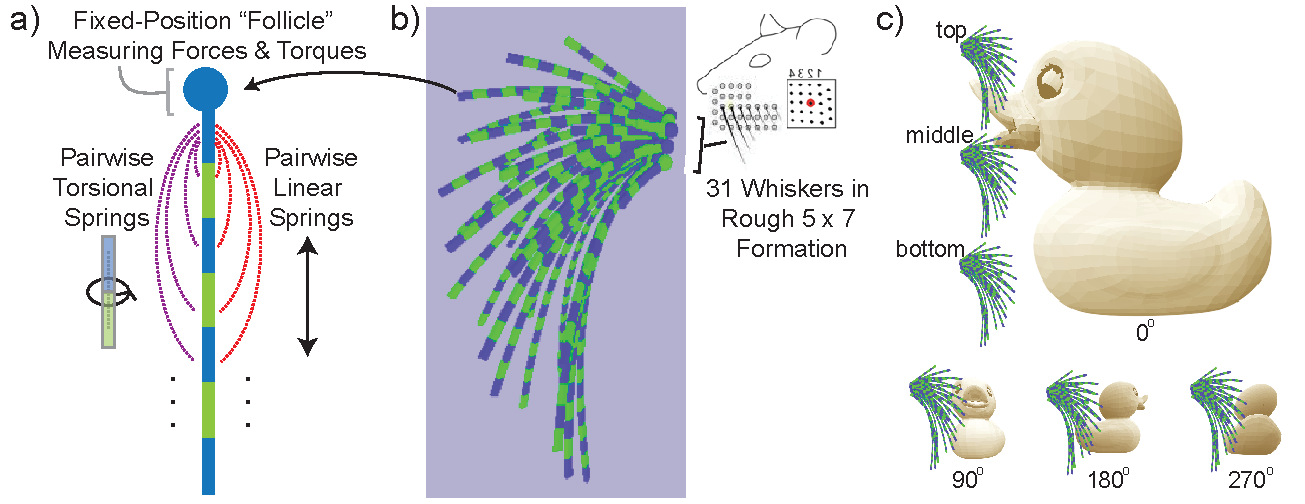
\includegraphics [width=\DefaultFigSize\linewidth]{figures/whiskers.pdf}
\vspace{-3mm}
\caption{\footnotesize{\textbf{Dynamic Three-Dimensional Whisker Model:} \textbf{a.} Each whisker element is composed of a set of cuboid links. 
The follicle cuboid has a fixed location, and is attached to movable cuboids making up the rest of the whisker. 
Motion is constrained by linear and torsional springs between each pair of cuboids. 
The number of cuboid links and spring equilibrium displacements are chosen to match known whisker length and curvature~\cite{Towal2011}, while damping and spring stiffness parameters are chosen to ensure mechanically plausible whisker motion trajectories.  
\textbf{b.} We constructed a 31-whisker array, arranged in a rough 5x7 grid (with 4 missing elements) on an ellipsoid representing the rodent's mystacial pad.  Whisker number and placement was matched to the known anatomy of the rat~\cite{Towal2011}.
\textbf{c.} During dataset construction, the array is brought into contact with each object at three vertical heights, and four 90$^{\circ}$-separated angles, for a total of 12 sweeps.  
The object's size, initial orientation angle, as well as sweep speed, vary randomly between each group of 12 sweeps. 
Forces and torques are recorded at the three cuboids closest to to the follicle, for a total of 18 measurements per whisker at each timepoint.}~\label{fig_whiskers}}
\vspace{-6mm}
\end{figure}

In order to provide our neural networks inputs similar to those of the rodent vibrissal system, we constructed a physically-realistic three-dimensional (3D) model of the rodent vibrissal array (Fig. \ref{fig_whiskers}).  
To help ensure biological realism, we used an anatomical model of the rat head and whisker array that quantifies whisker number, length, and intrinsic curvature as well as relative position and orientation on the rat's face~\cite{Towal2011}.
We wanted the mechanics of each whisker to the reasonably accurate, but at the same time, also needed simulations to be fast enough to generate a large training dataset.   
We therefore used the Bullet~\cite{wiki:bullet}, an open-source real-time physics engine used in many video games. 

\textbf{Statics.} Individual whiskers were each modeled as chains of ``cuboid'' links with a square cross-section and length of 2mm.   
The number of links in each whisker was chosen to ensure that the total whisker length matched that of the corresponding real whisker (Fig. \ref{fig_whiskers} a).
The first (most proximal) link of each simulated whisker corresponded to the follicle at the whisker base, where the whisker inserts into the rodent's face. 
Each whisker follicle was fixed to a single location in 3D space.  
The links of the whisker are given first-order linear and rotational damping factors to ensure that unforced motions dissipate over time. 
To simplify the model, the damping factors were assumed to be the same across all links of a given whisker, but different from whisker to whisker.   
Each pair of links within a whisker was connected with linear and torsional first-order springs; these springs both have two parameters (equilibrium displacement and stiffness). 
The equilibrium displacements of each spring were chosen to ensure that the whisker's overall static shape matched the measured curvature for the corresponding real whisker.  
Although we did not specifically seek to match the detailed biophysics of the whisker mechanics (e.g. the fact that the stiffness of the whisker increases with the 4th power of its radius),   
we assumed that the stiffness of the springs spanning a given length were linearly correlated to the distance between the starting position of the spring and the base, roughly capturing the fact that the whisker is thicker and stiffer at the bottom~\cite{Hartmann:2015}.

The full simulated whisker array consisted of 31 simulated whiskers, ranging in length from 8mm to 60mm (Fig. \ref{fig_whiskers}b). 
The fixed locations of the follicles of the simulated whiskers were placed on a curved ellipsoid surface modeling the rat's mystacial pad (cheek), with the relative locations of the follicles on this surface obtained from the morphological model~\cite{Towal2011}, forming roughly a $5\times7$ grid-like pattern with four vacant positions.

\textbf{Dynamics.} Whisker dynamics are generated by collisions with moving three-dimensional rigid bodies, also modeled as Bullet physics objects.  
The motion of a simulated whisker in reaction to external forces from a collision is constrained only by the fixed spatial location of the follicle, and by the damped dynamics of the springs at each node of the whisker. 
However, although the spring equilibrium displacements are determined by static measurements as described above, the damping factors and spring stiffnesses cannot be fully determined from these data.  
If we had detailed dynamic trajectories for all whiskers during realistic motions (e.g. \cite{Quist2014}), we would have used this data to determine these parameters, but such data are not yet available.  

In the absence of empirical trajectories, we used a heuristic method to determine damping and stiffness parameters, maximizing the ``mechanical plausibility'' of whisker behavior. 
Specifically, we constructed a battery of scenarios in which forces were applied to each whisker for a fixed duration.  These scenarios included pushing the whisker tip towards its base (axial loading), as well as pushing the whisker parallel or perpendicular to its intrinsic curvature (transverse loading in or out of the plane of intrinsic curvature).  
For each scenario and each potential setting of the unknown parameters, we simulated the whisker's recovery after the force was removed, measuring the maximum displacement between the whisker base and tip caused by the force prior to recovery ($d$), the total time to recovery ($T$), the average arc length travelled by each cuboid during recovery ($S$), and the average translational speed of each cuboid during recovery ($v$).    
We used metaparameter optimization~\cite{bergstra2013hyperopt} to automatically identify stiffness and damping parameters that simultaneously minimized the time and complexity of the recovery trajectory, while also allowing the whisker to be flexible.   
Specifically, we minimized the loss function $0.025S + d + 20T - 2v,$ where the coefficients were set to make terms of comparable magnitude.   
The optimization was performed for every whisker independently, as whisker length and curvature interacts nonlinearly with its recovery dynamics.   



